\newcommand{\template}{template}
\documentclass[listing,syntax,swedish]{\template/thesis}

\usepackage{amsmath}
\usepackage{subfig}
\begin{document}

% Title page

\def\TITLE{Implementering av en Lua-parser}
\def\SUBHEADING{}
\def\LEVEL{Examensarbete}
\def\PROGRAMME{Informationsteknik}
\def\UNIVERSITY{Arcada}

% Global (No translation)
\def\AUTHOR{Oskar Schöldström}
\def\IDENTIFICATION{12910}
\def\SUPERVISOR{Göran Pulkkis}
\def\COMMISSIONEDBY{}
\def\DATEACCEPTANCE{}
\def\DATE{\the\year}
\def\PAGECOUNT{73}
% \def\PAGECOUNT{\pageref{LastPage}}

% English
\addto\captionsenglish{%
  \def\TITLE{Implementing a Lua parser}
  \def\PROGRAMME{Information and Media Technology}
  \def\LEVEL{Degree Thesis}
  \def\KEYWORDS{Parsing, Recursive descent parser, Syntactic analysis, Lexical analysis, Metalanguage, JavaScript, Lua}
}

% Swedish
\addto\captionsswedish{%
  \def\TITLE{Implementering av en Lua parser}
  \def\PROGRAMME{Informations- och medieteknik}
  \def\LEVEL{Examensarbete}
  \def\KEYWORDS{Parsning, Rekursivt nedstigande parser, Syntaktisk analys, Lexikal analys, Metaspråk, JavaScript, Lua}
}

% Finnish
\addto\captionsfinnish{%
  \def\TITLE{Lua-parserin toteutus}
  \def\PROGRAMME{Informaatio- ja mediatekniikka}
  \def\LEVEL{Opinnäyte}
  \def\KEYWORDS{}
}


% Preamble stuff
\maketitle

\begin{abstract}{swedish}
  a  a \\
\end{abstract}

\begin{abstract}{english}
  a  a \\
\end{abstract}

\begin{abstract}{finnish}
  Lorem ipsum dolor sit amet, consectetur adipiscing elit. Maecenas molestie, nisi sed consectetur tincidunt, ante libero euismod nulla, eget commodo ligula purus eu nibh. Ut enim risus, congue sed viverra ut, tempor vel velit. Quisque consectetur tincidunt scelerisque. Donec nec mollis leo. Donec laoreet purus a massa ultrices egestas. Ut quis neque nisi. In hac habitasse platea dictumst. Suspendisse suscipit, ante eget venenatis molestie, elit nulla aliquam ligula, sit amet consectetur tortor magna eu ipsum. Pellentesque tempor tincidunt arcu, eget ultrices lorem commodo a.
\end{abstract}

\tableofcontents

\thispagestyle{empty}
\listoftables
\listoffigures
\clearpage


% Content
% \thispagestyle{empty}
%\addcontentsline{toc}{section}{Förkortningar och definitioner}
% \section*{Förkortningar}

\begin{tabular}{l l}
  API & Application Programming Interface \\
  AST & Abstract Syntax Tree \\
  ASCII & The American Standard Code for Information Interchange \\
  BNF & Backus-Naur Form \\
  EBNF & Extended Backus-Naur Form \\
  EOF & End-of-file \\
  GCC & The GNU Compiler Collection \\
  LL & Left to right, Leftmost derivation \\
  LR & Left to right, Rightmost derivation \\
  LALR & Look-Ahead Left to right, Rightmost derivation
\end{tabular}

\clearpage

% \addcontentsline{toc}{section}{Förord}
% \section*{Förord}
\thispagestyle{empty}

....

% \clearpage

\section{Inledning}

Det existerar ett flertal olika parser-arkitekturer i dagens kompilatorer.
Vissa använder sig av maskingenererad kod medan andra implementerar
komponenten manuellt. Beroende på komplexiteten av det kompilerade språkets
syntax påverkas även komplexiteten av parser implementationen upp till att
vissa implementationer väljer att inte vara fullständiga.

Rapporten utgår från att läsaren har kunskap inom programmering i allmänhet
samt en förståelse av JavaScript syntax.

\subsection{Målsättning}

Målet med detta examensarbete är att redogöra för hur ett programmeringsspråk
är uppbyggt och hur parsningen av dess syntax implementeras. Varför är vissa
språk svårare att parsa än andra? Vad är orsaken till att vissa kompilatorer
implementerar parser-komponenten manuellt medan andra använder en
maskingenererad komponent? Hur utförs implementationen av en parser i
praktiken och hur komplicerat är det? Detta är frågor som examensarbetet ämnar
besvara.

\subsection{Utförande}

Teoridelen av detta arbete redogör för hur programmeringsspråk är uppbyggt
samt hur de huvudsakliga parsning-arkitekturerna fungerar och används.

Den praktiska delen använder denna teori för att implementera en handskriven
Lua-parser i JavaScript. I kapitel 6 utförs en prestanda analys och parserns
väsentliga flaskhalsar avlägsnas. Orsaken till att JavaScript valts som
implementationsspråk är att i framtiden kunna använda parsern som ett
analyseringsverktyg i en nätbaserad kodredigerare.

För att upprätthålla en hög kvalitet på implementationen har diverse
kvalitetssäkringar gjorts upp. Över 500 funktionstest har skapats med hjälp av
kodgenerering och manuell verifiering. Testen baserar sig på Yueliang
projektets testsvit. Med dessa test har ett flertal fel korrigerats och
implementationen har i nuläget en kodtäckning på 100\%.

Funktionstest, mätning av kodtäckning, test för funktionskomplexitet samt en
statisk kodanlys körs innan varje uppdatering för att verifiera dess
kvalitet. Ytterligare används Travis kontinuerlig integrering för att
verifiera att utomstående uppdateringar håller standarden.

\subsection{Avgränsning}

Teorin om formella språk innehåller enbart det som krävs för att förstå senare
kapitel. Ytterligare presenteras enbart tekniker som är anses vara aktuella
för parser-implementationen eller Lua språket. Till detta hör inte senare
kompilatorskeden såsom semantisk analys eller kodgenerering.

% vim: set tw=78:ts=2:sw=2:et:fdm=marker:wrap:wm=78:ft=tex
% vim: spell spelllang=sv

\clearpage
\section{Språkteori}

För att en dator skall ha möjlighet att förstå innebörden i ett uttryck krävs
det att uttrycket är uppbyggt med en konsekvent utformning av såväl dess
syntax och dess semantik. Detta krav existerar inte i naturliga språk som
svenska utan existerar för en specifik typ av språk, de formella språken.
Formella språk är uppbyggda enligt matematiska regler som definierar språkets
alfabet och hur alfabetsymboler kan kombineras för att skapa uttryck. Teorin
härstammar från språkvetenskap men har idag en stor betydelse inom
datavetenskap eftersom den utnyttjas för att konstruera programmeringsspråk
\citep[s. 41]{sm09}.

\subsection{Backus-Naur Form}

Inom datavetenskap är syntax den kombination av tecken som är giltig för att
skapa ett uttryck. Uttryckets funktion kan variera, t.ex. kan funktionen
vara en del av ett flöde som skapar ett datorprogram, eller enbart ett format
för att uttrycka konfigurationer. Processen att läsa denna syntax och granska
om den är giltig kallas syntaktisk analys eller parsning.

När man beskriver syntaxen av ett språk använder man sig av ett metaspråk för
att definiera de syntaktiska regler man är tillåten att använda. Det finns ett
flertal metaspråk men ett av de vanligaste inom programmeringsspråk är
Backus-Naur Form (BNF) \citep[s. 27]{gd08}. Notationen är uppbyggd enligt
produktionsregler som var för sig definierar en tillåten sammansättning av
teckensträngar som kallas terminaler eller icke-terminaler. Terminaler är
teckensträngar som inte refererar vidare till andra teckensträngar medan
icke-terminaler är sekvenser av terminaler som bildar giltiga
produktionsregler eller språkliga meningar. Ytterligare existerar vissa
symboler för att uttrycka vilken typ av sammansättningsfunktion är tillåten.

BNF i sig existerar dessutom i flera varianter där vissa varianter är strikta och
ämnade att läsas av maskiner, medan andra varianter försöker visualisera elementen
för en mänsklig läsare. Extended BNF (EBNF) som är en utökad variant av den
ursprungliga BNF-notationen skriver icke-terminaler inom vinkelparentes i
formen ${\langle}regel{\rangle}$. En produktionregels namn, som är en
icke-terminal,
skrivs längst till vänster följt av symbolerna $::=$ samt själva regeln.
Terminalerna skrivs med fet stil och sammansättningarna skrivs med normal
stil samt regelns specifika syntax. De vanliga funktionerna är alternering, som
skrivs med ett lodrätt streck ($|$) mellan alternativen, repetition som skrivs
med en vågparentes ($\{ \ldots \}$) omkring uttrycket och slutligen
valfrihet som skrivs med en hakparentes ($[ \ldots ]$) runt uttrycket
\citep[s. 28]{gd08}. Dessa är de viktigaste elementen i BNF men det existerar
även övriga funktioner för bl.a. bekvämlighet och läsbarhet.

\subsection{Chomskyhierarkin}

När man skriver grammatiken till ett språk beaktar man alltid vilka
typer av regler man vill tillåta i specifikationen. Utgående från valet man
gör kommer grammatiken och därmed också språket tillhöra en av fyra språkliga
delmängder som sträcker sig från enkel till komplicerad \citep[s. 19]{gd08}
enligt figur~\ref{fig:chomskyhierarki}.

\begin{figure}[ht]
  \includegraphics[width=5cm]{figures/output/chomsky.pdf}
  \caption{De fyra nivåerna i Chomskyhierarkin}
  \label{fig:chomskyhierarki}
\end{figure}

Denna indelning kallas för Chomskyhierarkin och används bl.a. för att ta reda
på vilken typ av automat som krävs för att läsa språket. Typen av automat
påverkar komplexiteten av implementationen samt tidsmängden som krävs för att
läsa språket.

Delmängderna börjar från den enklaste typen, reguljär grammatik. Den
reguljära grammatiken är sedan en delmängd av den kontextfria grammatiken som i
sin tur är delmängd till den kontextkänsliga grammatiken. Slutligen tillhör
alla de tidigare nämnda även den obegränsade grammatiken som kan
beskriva alla grammatiker vilka accepteras av en Turingmaskin.

De två huvudsakliga grupperna i dagens programmeringsspråk är dock de två
innersta, reguljära grammatiker samt kontextfria grammatiker \citep[s.
100]{sm09}. Dessa är möjliga att skriva både för hand och av maskiner och har
därför blivit mycket vanliga i design av programmeringsspråk. Majoriteten av
språk använder sig av en kontextfri syntax. Ett undantag är C++ vars
uttryck inte kan definieras enbart utgående från syntaxen utan kräver också en
semantisk analys av ett flertal uttryck. På grund av detta är C++ grammatiken
kontextkänslig och därmed också svår att parsa. I flera fall har
parser-implementationer valt att ignorera mångtydigheterna på grund av deras
komplexitet och deras obetydliga användning \citep[s. 2]{rt05}.

\subsubsection{Reguljär grammatik}

Den innersta delmängden i Chomskyhierarkin är reguljär grammatik och kan uttryckas
enbart m.h.a. reglerna sammanfogning, alternering och repetition. I
programmeringsspråk används ofta en reguljär grammatik för att identifiera
s.k. lexikala element och går att läsa med en ändlig automat \citep[s.
100]{sm09}.

För att beskriva alla variationer av ett naturligt tal i en kalkylator kan man
använda sig av EBNF grammatiken i figur~\ref{fig:reg}. Ett tal definieras som
alterneringen av ett heltal och ett reellt tal. Ett heltal måste bestå av
minst en siffra medan ett reellt tal kan bestå av antingen ett heltal samt en
exponent eller ett decimaltal och en valfri exponent. Detta innebär att
uttrycken \textit{0.14E-2} och \textit{3} är giltiga medan uttrycket
\textit{222e} inte är giltigt eftersom en exponent måste avslutas med ett
heltal. Dessutom måste man tänka på att ett giltigt decimaltal i en riktig
kalkylator inte nödvändigtvis behöver börja med en siffra utan kan börja med
en punkt, dock måste det antingen börja med en siffra eller avslutas med en
siffra eftersom ett uttryck enbart innehållande en punkt inte kan räknas som
giltigt. Alla dessa regler kan bli komplicerade att hålla reda på och därför
underlättar det att arbeta med BNF notationer för att inte mista giltiga
uttryck.

\begin{figure}[ht]
  \begin{grammar}
    \singlespace\small%
    \fontfamily{lmr}\selectfont

    <tal> ::= ["-"] (<heltal> | <reellt tal>)

    <heltal> ::= <siffra> \{<siffra>\}

    <reellt tal> ::= <heltal> <exponent>
      \alt <decimaltal> [<exponent>]

    <decimaltal> ::= <heltal>.<heltal>

    <exponent> ::= ("e" | "E") ["+" | "-"] <heltal>

    <siffra> ::= "0" | "1" | "2" | "3" | "4" | "5" | "6" | "7" | "8" | "9"

  \end{grammar}
  \caption{EBNF grammatik för ett tal.}
  \label{fig:reg}
\end{figure}

\subsubsection{Kontextfri grammatik}

Tillåter man ytterligare rekursion i en giltig regel är grammatiken inte
längre reguljär, utan klassas som en kontextfri grammatik och måste läsas av
en s.k. \textit{``push-down''} automat ofta kallad parser. Skillnaden från en
ändlig automat är att \textit{``push-down''} automaten har en stack val av
tillstånd \citep[s.  100]{sm09}. Rekursion innebär att en produktionsregel kan
innehålla sig själv som en icke-terminal i regeldefinitionen. Denna
funktionalitet är användbar när ett uttryck skall vara flexibelt, exempelvis i
en kalkylator var ett uttryck kan bestå av ett tal, en matematisk operation
samt en oändlig uppsättning av dessa.

Figur~\ref{fig:cfg} visar ett exempel på en kalkylator som kan uttrycka alla
dessa funktionaliteter genom att rekursivt hänvisa till sig själv och därmed
tillåta uttryck så som \mbox{\textit{1 + (2 / 7) * -3}}.

\begin{figure}[ht]
  \begin{grammar}
    \singlespace\small%
    \fontfamily{lmr}\selectfont

    <uttryck> ::= <tal>
      \alt "(" <uttryck> ")"
      \alt <uttryck> <operator> <uttryck>

    <operator> ::= + | - | * | /

  \end{grammar}
  \caption{EBNF grammatik för en kalkylator.}
  \label{fig:cfg}
\end{figure}

% vim: set tw=78:ts=2:sw=2:et:fdm=marker:wrap:wm=78:ft=tex
% vim: spell spelllang=sv

\clearpage
\section{Parsning}

Implementeringen av ett programmeringsspråk finns i flera varianter och en
vanlig sådan är kompilatorn. Denna implementation läser input och producerar
sedan ett körbart program utgående från de instruktioner den fått.  Själva
processen av kompilering består av flera faser och komponenter. Den första
komponenten är en parser som läser input och konstruerar en maskinläslig
struktur utgående från den grammatik som givits. Vid detta skede bryr sig
programmet inte ännu om vad som skall göras utan den försöker enbart
identifiera de olika reglerna och granska att dess syntax är korrekt. Parsern
körs normalt som en komponent inne i en tolk vars funktion i sin tur är att
förstå och tolka innebördet hos en regel. När parsern är klar med sin analys
returnerar den strukturen till tolken som i sin tur returnerar sin modifierade
version av strukturen tillbaka till huvudkomponenten, kompilatorn. Kompilatorn
fungerar som en översättare som slutligen genererar den kod som datorns
processor kan förstå. En översikt av dessa komponenter och dess funktioner
visas i figur~\ref{fig:compiler} \citep[s. 16]{pt10}.

\begin{figure}[ht]
  \includegraphics[width=\textwidth]{figures/output/language-stages.pdf}
  \caption{Översikt av komponenterna i en kompilator.}
  \label{fig:compiler}
\end{figure}

Parsningsprocessen kan delas upp i två skilda faser, först en s.k.
lexikal analys som identifierar lexikala element, som kallas tokens. Tokens
är identifierbara teckensträngar med speciell betydelse. De kategoriseras
enligt typer såsom nyckelord, konstanter, parametrar osv. \citep[s. 6]{aa06}.

Den andra fasen som sker efter identifieringen av tokens är den syntaktiska
analysen där elementen sammansätts till helhetsuttryck granskat enligt
grammatikens produktionsregler.

\subsection{Lexikal analys}

Eftersom elementen i en lexikal analys kan beskrivas med en reguljär grammatik
använder man sig ofta av en ändlig automat för att läsa den. Denna typ av
automat brukar man kalla för lexer. Automaten börjar i ett specifikt startläge
var den väntar på ett tecken att läsa. När ett tecken läses går den genom en
serie alterneringar för att minska mängden slutgiltiga lösningar. När därpå
följande tecken läses in fortsätter den att härleda sig vidare tills den når
en slutgiltig lösning, eller alternativt inte känner igen elementet och skapar
ett felmeddelande. När lösningen är hittad skickar lexern det identifierade
elementet tillbaka till parsern och återgår till sitt utgångsläge för att
vänta på nästa tecken.  På detta sätt kan lexern, som har en effektiv
algoritm, avlägsna onödig information såsom mellanslag och kommentarer för att
sedan ge uttryckets egentliga element vidare till parsern som nu enkelt vet om
en teckensträng är en nyckelordsterminal eller ett tal \citep[s.  51]{sm09}.
Ett lexikaliseringsexempel visas i figur~\ref{fig:lexing}.

\begin{figure}[ht]
  \begin{alltt}
\boxkeyword{if} \boxint{2} \boxpunct{+} \boxint{1} \boxpunct{>} \boxint{3} \boxpunct{==} \boxkeyword{false} \boxkeyword{then}
  -- en kommentar
  \boxkeyword{print} "\boxstring{foo}"\boxpunct{;}
\boxkeyword{end}
  \end{alltt}
  \caption{Ett lexikaliseringsexempel på en if-sats skriven i Lua.
    Blanksteg samt kommentarer ignoreras och tokentyperna är nyckelord, tal,
    specialsymbol och teckensträng.}
  \label{fig:lexing}
\end{figure}

\subsection{Syntaktisk analys}

Processen att parsa input och validera dess syntax enligt en kontextfri
grammatik kallas syntaktisk analys eller enbart parsning. Detta görs
vanligtvis i kombination med en lexikal analys för att förenkla
implementation men kan också genomföras direkt på input \citep[s. 8]{aa06}.

Analysen kombinerar de tokens som identifierats en efter en och försöker hitta
en giltig produktionsregel för kombinationen. Om en produktionsregel
identifierats förväntas alla tokens överensstämma med regeldefinitionens
terminaler och icke-terminaler. Visar det sig att en token inte överensstämmer
skapas ett felmeddelande.

Vid implementationen av en kompilator avbryts parsningen när ett fel
påträffats eftersom syntaxen inte är giltig. Vissa andra implementationer
såsom \textit{``syntax highlighters''} i textredigerare försöker hoppa över
produktionsregeln och fortsätta med nästa eftersom detta ger en bättre
användarupplevelse.

\subsection{Syntaxrepresentation}

Allteftersom produktionsregler parsats i.o.m. en syntaktisk analys skapas en
maskinförståelig representation av dess innehåll. Lättast är det att tänka sig
denna representation som en trädstruktur trots att den inte nödvändigtvis
behöver vara det.

\begin{figure}[ht]
  \includegraphics[width=8cm]{figures/output/tree.pdf}
  \caption{En trädrepresentation av en if-sats skriven i Lua.}
  \label{fig:syntaxtree}
\end{figure}

Varje nod i trädet representeras av en produktionsregel. Löv-noderna är
terminaler (figur~\ref{fig:syntaxtree}). Terminaler såsom \textit{if}, och
\textit{else} utelämnas ofta i en praktisk implementation eftersom de kan
knytas som attribut till en nod \citep[s. 49]{sm09}.

Representationen skapas i den syntaktiska analysatorn när en produktionsregel
identifierats och kan sedan användas i senare skeden såsom i en semantisk
analysator eller kodoptimeringskomponent.

Trädstrukturerna varierar beroende på syftet av parsern. Kompilatorer vill
att de skall vara så nära maskinkod som möjligt medan andra verktyg såsom
statiska kodanalysatorer vill att de ska vara på en högre nivå \citep[s.
6]{pt10}.

En vanlig representationsform på en högre nivå är ett abstrakt syntaxträd
(AST).  Detta är verkligen uppbyggt såsom ett träd enligt vad beskrivits
hittills. Karaktärsdrag av ett AST är att det är kompakt, enkelt att förflytta
sig genom och betydelsefullt. Exempelvis kan varje nod existera som ett objekt
i en klass namngiven efter produktionsregeln \citep[s 77]{pt10}.

\subsection{Parsertyper}

Beroende på grammatiken av ett språk krävs det olika algoritmer för att kunna
parsa den. Den s.k. Early-algoritmen kan parsa alla typer av kontextfria
grammatiker i $O(n^3)$ tid, där n är inputlängd \citep[s. 67]{sm09}. De
flesta parsers behöver dock inte en så generell grammatik utan kan parsas i
$O(n)$ tid med hjälp av \textit{``uppifrån-och-ner''}-algoritmer eller
\textit{``nerifrån-och-upp''}-algoritmer. Det existerar ytterligare algoritmer
för olika delmängder av kontextfria grammatiker men de vanligaste bygger på
någon av dessa \citep[s. 61]{aa06}.

När man beskriver en parser nämner man ofta hur långt fram den kan se innan
den gör ett beslut av vilken produktionsregel den skall följa, hur många s.k.
\textit{``lookahead''}-tokens den har. Detta antal skriver man inom en
parentes efter parsertypens namn. Exempelvis skulle den s.k. LL-parsern med 2
\textit{``lookahead''}-tokens skrivas LL(2) \citep[s. 69]{sm09}.

\subsubsection{LL-parser}

LL-parsers härleder regler från vänster och använder sig av
\textit{``uppifrån-och-ner''}-algoritmen. Parsern klarar av en mindre delmängd
av kontextfria grammatiker och man använder benämningen LL-grammatik för att
uttrycka den delmängd som en LL-parser kan parsa.

En LL-parser går att skriva för hand eftersom den i allmänhet följer en logisk
tankegång. Den börjar från en rot-regel och arbetar sig sedan neråt
med hjälp av hjälp av jämföra terminaler från vänster, likt en ändlig
automat. När alla alternativa lösningar uteslutits förväntar sig parsern att
löv-reglerna skall passa in en efter en.

\subsubsection{LR-parser}

LR-parsers härleder regler från höger och använder sig av
\textit{``nerifrån-och-upp''}-algoritmen. Denna typ av parser klarar av att
analysera en större delmängd grammatiker än t.ex. LL-parsers och är därmed mer
vanlig i programvara som genererar parsers \citep[s. 61]{aa06}.

LR-parsers genereras huvudsakligen av maskiner eftersom de är svårare att
visualisera. Dessa parsers börjar med att läsa löv-reglerna, alltså de minsta
identifierbara reglerna och ansluter dem sedan till varandra fram till det att
den nått en slutgiltig rot-regel \citep[s. 67]{sm09}.

En steg för steg jämförelse mellan LR- och LL-parserns algoritmer visas i
figur~\ref{fig:ll-vs-lr}.

\begin{figure}[ht]
  \begin{minipage}[t]{0.5\textwidth}
    \Tree [.{\textit{\hspace*{0.5cm}Uttryck}}
  !\qsetw{1.5cm}
]
\\

\Tree [.{\textit{Uttryck}}
  \textbf{2}
  \textbf{+}
  \textit{uttryck}
  !\qsetw{1.5cm}
]
\\

\Tree [.{\textit{Uttryck}}
  \textbf{2}
  \textbf{+}
  [.{\textit{uttryck}}
    \textbf{3}
    \textbf{-}
    \textit{uttryck}
    !\qsetw{1.5cm}
  ]
  !\qsetw{1.5cm}
]
\\

\Tree [.{\textit{Uttryck}}
  \textbf{2}
  \textbf{+}
  [.{\textit{uttryck}}
    \textbf{3}
    \textbf{-}
    [.{\textit{uttryck}}
      \textbf{4}
      !\qsetw{1.5cm}
    ]
    !\qsetw{1.5cm}
  ]
  !\qsetw{1.5cm}
]

  \end{minipage}%
  \begin{minipage}[t]{0.5\textwidth}
    \textbf{2}

\textbf{2} \textbf{+}

\textbf{2} \textbf{+} \textbf{3}

\textbf{2} \textbf{+} \textbf{3} \textbf{-}

\textbf{2} \textbf{+} \textbf{3} \textbf{-} \textbf{4}
\\

\textbf{2} \textbf{+} \textbf{3} \textbf{-} \Tree [.{\textit{uttryck}}
  \textbf{4}
]
\\

\textbf{2} \textbf{+} \Tree [.{\textit{uttryck}}
  \textbf{3}
  \textbf{-}
  [.{\textit{uttryck}}
    \textbf{4}
  ]
]
\\

\Tree [.{\textit{Uttryck}}
  \textbf{2}
  \textbf{+}
  [.{\textit{uttryck}}
    \textbf{3}
    \textbf{-}
    [.{\textit{uttryck}}
      \textbf{4}
    ]
  ]
]

  \end{minipage}%
  \caption{Steg för steg parsning av ett matematiskt uttryck med en
    ``uppifrån-och-ner''-algoritm (vänster) och en
    ``nerifrån-och-upp''-algoritm (höger).}
  \label{fig:ll-vs-lr}
\end{figure}

\subsubsection{LALR-parser}

LALR-parsern baserar sig på en LR(0)-parsers struktur men med stöd för
\textit{``lookahead''}-tokens. Skillnaden mellan LR-parsers med stöd för
\textit{``lookahead''}-tokens och LALR-parsern är antalet tillstånd
\textit{``push-down''}-automaten har.  Eftersom LALR-parsern kräver färre
tillstånd och dessutom kräver mindre minne kan den ses som en förenklad och
mer effektiv version \citep[s. 266]{aa06}.

\subsubsection{Rekursivt nedstigande parser}

En annan typ av parser som använder sig av
\textit{``uppifrån-och-ner''}-algoritmen är den rekursivt nedstigande parsern.
Denna parsertyp klarar av att parsa LL-grammatik och är därför vanlig för
handskrivna parsers. Istället för att utnyttja en automat fungerar den genom
att knyta varje icke-terminal i grammatiken till en egen funktion som ansvarar
för att identifiera dess löv i grammatiken. För varje icke-terminal i sin egen
regel anropar den rekursivt vidare dess funktioner fram till det att rot
funktionen får hela syntaxträdet returnerat \citep[s. 24]{pt10}.

Flödet av en rekursivt nedstigande parser visas i
figur~\ref{fig:recursivedescent} där varje nod symboliserar en funktion.
En röd pil symboliserar dess funktionsanrop medan en blå pil symboliserar
funktionens returnering.

\begin{figure}[ht]
  \includegraphics[width=12cm]{figures/output/recursivedescent.pdf}
  \caption{Flöde av en rekursivt nedstigande parser steg för steg.}
  \label{fig:recursivedescent}
\end{figure}

\subsection{Eliminering av mångtydighet}

\subsubsection{Vänsterrekursion}

Ett vanligt problem med grammatiken i en parser med \textit{``uppifrån-och-ner''}
algoritmen är vänsterrekursion. Detta innebär att produktionsregel använder
sig själv som icke-terminal längst till vänster i sammansättningen. När
detta inträffar kommer implementationen att fastna i en oändlig upprepning.
För att implementera en LL-parser måste man därför eliminera vänsterrekursion.

Exempelvis är produktionsregeln för kalkylatorn i figur~\ref{fig:cfg} på sida
\pageref{fig:cfg} vänsterrekursiv.

\setlength{\grammarindent}{5em}
\begin{grammar}
  \singlespace\small%
  \fontfamily{lmr}\selectfont
  <uttryck> ::= <tal>
    \alt "(" <uttryck> ")"
    \alt <uttryck> <operator> <uttryck>
\end{grammar}

Genom att expandera rekursionen i alla existerande villkor som nya villkor får
vi:

\setlength{\grammarindent}{5em}
\begin{grammar}
  \singlespace\small%
  \fontfamily{lmr}\selectfont
  <uttryck> ::= <tal>
    \alt "(" <uttryck> ")"
    \alt <tal> <operator> <uttryck>
    \alt "(" <uttryck> ")" <operator> <uttryck>
\end{grammar}

Detta beskriver fortfarande en identisk grammatik och följande steg är att
förenkla uttrycket med en ny produktionsregel som utnyttjar $\epsilon$, en
symbol för att representera ett tomt värde.

\setlength{\grammarindent}{5em}
\begin{grammar}
  \singlespace\small%
  \fontfamily{lmr}\selectfont
  <uttryck> ::= <tal> <uttryck'>
    \alt "(" <uttryck> ")" <uttryck'>

  <uttryck'> ::= <tal>
    \alt "(" <uttryck> ")"
    \alt <operator> <uttryck>
    \alt $\epsilon$
\end{grammar}

Grammatikens funktion är fortfarande identisk men vänsterrekursionen som är
omöjlig att utföra i en \textit{``uppifrån-och-ner''} algoritm är eliminerad.

En förenklad matematisk regel som kan användas för att eliminera
vänsterrekursionen $A \rightarrow A\alpha\;|\;\beta$ är \citep[s. 212]{aa06}:
\begin{align*}
A &\rightarrow \beta A^\prime \\
A^\prime &\rightarrow \alpha A^\prime\;|\;\epsilon
\end{align*}

\subsubsection{Vänsterfaktorering}

Ytterligare ett problem \textit{``uppifrån-och-ner''}-algoritmen är
produktionsregler där två villkor påminner om varandra i början av
definitionen.

Exempelvis behövs en obestämd mängd \textit{``lookahead''}-tokens för att
identifiera det korrekta villkoret i följande produktionsregel:

\setlength{\grammarindent}{5em}
\begin{grammar}
  \singlespace\small%
  \fontfamily{lmr}\selectfont
  <if> ::= "if" <uttryck> "then" <block> "else" <block> "end"
    \alt "if" <uttryck> "then" <block> "end"
\end{grammar}

Med hjälp av vänsterfaktorering kan vi omvandla regeln till:

\setlength{\grammarindent}{5em}
\begin{grammar}
  \singlespace\small%
  \fontfamily{lmr}\selectfont
  <if> ::= "if" <uttryck> "then" <block> <else>

  <else> ::= "else" <block> "end"
    \alt "end"
\end{grammar}


Den matemtiska regeln för liknande uttryck i formen $A \rightarrow
\alpha\beta_1\;|\;\alpha\beta_2 $ är \citep[s. 214]{aa06}:
\begin{align*}
A &\rightarrow \alpha A^\prime \\
A^\prime &\rightarrow \beta_1\;|\;\beta_2
\end{align*}

\subsection{Vidareutveckling av parsertyper}

\subsubsection{Backtracking}

I vissa fall är det användbart att inte ha en begränsad mängd
\textit{``lookahead''}-tokens och då kan man använda sig av en metod som heter
\textit{``backtracking''} förutsatt det handlar om en rekursivt nedstigande
parser.

Implementationen av en \textit{``backtracker''} görs genom att markera
positionen var en mångtydighet uppstår och sedan välja ett regelalternativ.
När alternativet bevisats vara korrekt eller inkorrekt återgår parsern till
den markerade positionen. Om ett felmeddelande skapats försöker parsern med
följande alternativ och repeterar detta fram till att en regel visar sig vara
korrekt varefter den påbörjar den egentliga parsningen utan att markera
positionen \citep[s. 57]{pt10}.

För att uttrycka att en parser kan se en obegränsad mängd tokens framåt anger
man antalet som k i LL(k).

\subsubsection{Packrat parsning}

En nackdel med den tidigare nämnda \textit{``backtracking''}-metoden är att
parsern alltid måste återgå till det tidigare tillståndet och därefter påbörja
en andra parsning av regeln. Detta ökar den tidsmängd som krävs för att parsa
ett inputvärde.

Packrat parsning är en annan typ av parser vars metod går att implementera för
en rekursivt nedstigande parser. Den fungerar likt
\textit{``backtracking''}-metoden men skiljer sig genom att memorera
resultatet av parsningsträdet samt positionen var parsningen avslutades. När
parsern återgår till det tidigare tillståndet granskar den om parsningen var
framgångsrik. Om den visar sig vara, använder parsern sig av det redan
memorerade parsningsträdet och hoppar vidare till positionen där parsningen
avslutades.

\subsection{Parser-generatorer}

Att implementera en parser för hand är en tidskrävande och felbenägen process.
Produktionsregler påminner mycket om varandra och repetitionen att
implementera varje regel blir en långdragen uppgift med möjlighet för
introduktion av fel vid varje steg. På grund av detta har det blivit populärt
att använda en s.k. parser-generator som förser programmeraren med en färdig
parser-implementation utgående från en given grammatik \citep[s. 26]{pt10}.

Med hjälp av en parser-generator kan implementatören upprätthålla grammatiken
av ett språk genom att skriva och modifiera en BNF-liknande syntax istället
för den egentliga koden. Detta har stora fördelar om grammatiken inte är helt
stabil eftersom enbart några rader behöver korrigeras vid förändringar. För
ett språk med en stabil grammatik existerar fördelarna endast vid
implementationsskedet och kan vara en nackdel i situationer som felsökning och
skapandet av läsbara felmeddelanden för syntaxfel \citep[s. 175]{bf09}.

Uppdelningen av genererade parsers och handskrivna parsers är delad, de flesta
språk använder sig av en genererad parser men några såsom C-språkets GCC \citep{gcc}
samt Luas egna parser \citep{luaimp} har börjat från en genererad parser och
sedan övergått till en handskriven rekursivt nedstigande parser för utökad
funktionalitet.

Parser-generatorer existerar för flera språk samt för diverse grammatik- och
algoritmtyper. I detta kapitel kommer jag att presentera två
parser-generatorer som är vanliga i unix-system.

\subsubsection{Lex}

Lex är en generator för reguljära grammatiker skapad av Mike Lesk och
Eric Schmidt. Verktyget använder en egen grammatiksyntax för att
definiera produktionsregler i ett språk och generera sedan en lexer i C eller
Ratfor. För varje produktionsregel kan användaren definiera en åtgärd som
kommer att exekveras när en regel identifierats. Vanligen är detta C-kod för
att returnera värdet till en syntaktisk analysator. Eftersom Lex genererar kod
existerar funktionalitet för att inkludera valfri C-kod som kopieras till
resultatfilen. Detta kan användas till att inkludera bibliotek eller
definiera funktioner som produktionsreglerna använder \citep{lex}.

I figur~\ref{fig:lex} visas en enkel grammatikspecifikation som läser input
och identifierar variabeldeklarationer av strängar eller heltal samt ignorerar
blanksteg.

\begin{figure}[ht]
  \lstinputlisting[title="",keywords={printf,return,include,main}]%
    {figures/tex/lex.l}
  \caption{En Lex-specifikation för att identifiera variabeldeklarationer av
    strängar eller heltal.}
  \label{fig:lex}
\end{figure}

En fritt tillgänglig version av Lex är Flex som distribueras av bl.a.
GNU-projektet. I allmänhet är Flex-kompatibel med Lex och är därför ett
populärt alternativ \citep[s. 279]{bd92}.

\subsubsection{Yacc}

Eftersom de flesta programmeringsspråk använder sig av en kontextfri grammatik
är inte Lex verktyget tillräkligt utan man behöver ytterligare en syntaktisk
analysator. Yacc är en parser-generator för kontextfri grammatik skapad av
Stephen Johnson. Syntaxen för grammatikspecifikationen liknar mycket Lex.
Användaren definierar produktionsregler samt deras åtgärder men har nu
möjligheten att använda rekursion. Ytterligare bör man definiera en
lexikaliseringsfunktion, exempelvis \textit{yylex()}, samt vilka tokentyper
som existerar. Integreringen måste ske både i den valfria lexern och i
Yacc-specifikationen, t.ex. med en delad definitionsfil av tokens som lexern
returnerar och den Yacc-genererade parsern kan identifiera. Ett
pseudokod-exempel på ett språk som tillåter variabeldeklarationer av heltal
och strängar visas i figur~\ref{fig:yacc}. För att parsern skall fungera
måste logiken för \textit{input} samt lexikaliseringen av \textit{VARIABLE},
\textit{STRING}, \textit{INTEGER} och \textit{EQUAL_SIGN} definieras i lexer
koden.

GNU-projektet har även skapat en \textit{``copyleft''}-licenseriad version av Yacc som
heter GNU bison. Bison är i allmänhet kompatibel med Yacc-syntax och är därför
ett populärt alternativ \citep[s. 277]{bd92}.

\begin{figure}[ht]
  \lstinputlisting[title="",keywords={printf,return,include,main,do,while}]%
    {figures/tex/yacc.y}
  \caption{En Yacc-specifikation för variabeldeklarationer av heltal och
    strängar.}
  \label{fig:yacc}
\end{figure}

\subsubsection{Jison}

Jison är en JavaScript-programmerad parser-generator för både reguljära grammatiker
och kontextfria grammatiker. Verktyget använder samma koncept som Lex/Flex
samt Yacc/Bison och därmed är grammatik-specifikationen samma. Skillnaden är
att specifikationen kan innehålla grammatik för både lexern och den
syntaktiska analysatorn. Trots att det finns funktionalitet för att generera
både en lexer och en syntaktisk analysator tillåter Jison att användaren
utnyttjar en separat lexer som följer ett specificerat gränssnitt
\citep{jison}.

% vim: set tw=78:ts=2:sw=2:et:fdm=marker:wrap:wm=78:ft=tex
% vim: spell spelllang=sv

\clearpage
\section{Lua-parserns implementation}

Implementationen är indelad i fyra komponenter. När parsern startas börjar
en syntaktisk analysator parsa input från rot-noden.  Det första som görs är
ett anrop till den andra komponenten, lexern. Lexern läser input tecken för
tecken och tokeniserar värden som sedan returneras till den syntaktiska
analysatorn var den används för att välja produktionsregel. Utanför lexern
hanteras inte enskilda tecken utan enbart tokens.  Utöver dessa två
komponenter finns en separat uttrycksparser samt ett delegerare som producerar
ett syntaxträd vilket slutligen returneras till programmet som anropat parsern
i första hand.

\subsection{Lexer}

Lexern läser input enligt en reguljär grammatik och gör detta som en
deterministisk ändlig automat. När parsningen av en token börjar hämtas det
aktuella tecknet i input strängen och lexern går sedan genom en serie villkor
för att bestämma var en token slutar och av vilken typ den är. När en token
slutat har automaten nått sitt slutliga tillstånd och tokenvärdet returneras.
Slutligen återgår automaten till utgångsläget för att vänta på nästa
förfrågan.

Tokentyperna som lexern användar är: \textit{``End-of-file''} (EOF),
teckensträngs-litteral, nyckelord, identifierare, tal-litteral, symbol,
boolean samt nil. Dessa definieras som uppräkningsflaggor (enum flag) för att
kunna jämföras med bit operationer. När en token identifieras av lexern
returneras den som ett objekt med attribut för tokentypen, dess index-position
i input-teckensträngen, dess rad och kolumn i input samt dess tokenvärde.

\subsubsection{Blanksteg och kommentarer}

Eftersom blanksteg utgör 40\% av implementationens kod kan det konstateras att
lexern spenderar en väsentlig del av sin tid på blanksteg. Det första lexern
gör när den anropas är att anropa en funktion som ignorerar alla
blankstegstecken som hittas.

Eftersom token-objekt innehåller information om rad och kolumn i input
memoreras varje radförändringen i funktionen som ignorerar blanksteg.
Ytterligare lagras input-positionen när en rad påbörjas. När ett tokenobjekt
skapas subtraheras radens startposition från den nuvarande input-positionen
och bildar därmed kolumnen.

Kompilatorer kan ignorera kommentarer eftersom de inte innehåller semantiska
värden men eftersom målet med denna implementation är användning för
kodanalys sparas även kommentarer. Detta görs genom att söka efter
avgränsarsymbolen (\verb+--+) och lagra dess information i en separat tabell
som slutligen anknyts till det returnerade syntaxträdet.

\subsubsection{Identifierare och nyckelord}

Från och med Lua 5.2 kan variabelnamn, eller s.k. identifierare, endast bestå av
bokstäver, siffror och understreck i ASCII-uppsättningen. Ytterligare kan ett
variabelnamn inte börja med en siffra \citep{luaref}.

Nyckelord är terminaler med samma regler som identifierare och därmed kan de
använda samma logik för att avskilja giltiga tecken. En skillnad mellan
parser-implementationen och Lua-grammatiken är åtskiljandet mellan nyckelord
och datatyperna nil, boolean.

Med att granska grammatiken för tokentyperna kan det utläsas att enbart nil,
boolean, nyckelord samt identifierare kan börja med en bokstav. Eftersom
lexern arbetar tecken för tecken kan detta användas som en villkorsförgrening.
Om en ny token börjar med en bokstav måste det tillhöra någon av dessa fyra
tokentyper, ytterligare vet vi att tokentypen slutar där ett tecken inte är en
bokstav, en siffra eller ett understreck.

Implementationen av denna fögrerning görs genom att läsa ASCII-koden för
tecknet och granska om det är en bokstav eller ett understreck. Om testet
lyckas fortsätter lexern att acceptera tecken så länge som teckenkoden tillhör
serien för bokstäver, siffror och understreck. När testet misslyckas betyder
det att denna token tagit slut och nu kan lexern granska om värdet är lika med
ett boolean-värde, ett nil-värde, ett av nyckelorden eller inte tillhör någon
av dessa och därmed är en identifierare.

\subsubsection{Symboler}

Identifieringen av symboler implementeras med en serie switch- och
if-satser vilka granskar vilka tecken framåt i input tillhör en giltig
symbol. När den längsta möjliga symbolen identifieras returneras den.

Luas giltiga symboler är:
\begin{verbatim}
. .. ... : :: ; # = == > >= < <= ~= { } ( ) [ ] ^ % * / - +
\end{verbatim}

\subsubsection{Litteraler}

Lua stöder tal likt vanliga programmeringsspråk men har även stöd för
hexadecimaltal innehållande en valfri binär expontent. Implementationen läser
input och verifierar att talet är giltigt. När token-värdet identifierats
konverteras det till ett flyttal och returneras.

Teckensträngar i Lua börjar antingen med enkla citationstecken (\verb+'+)
eller dubbla citationstecken (\verb+"+) och samma avgränsarsymbol förväntas
innan raden tar slut. Lua tillåter dock att man inaktiverar en symbol såsom
citations- eller radbrytningstecken genom att använda ett omvänt snedstreck
(\verb+\+). En annan användning för det omvända snedstrecket är att definiera
en styrkodsekvens.  När lexern hittar ett snedstreck inom en
teckensträngslitteral granskas först giltiga styrkodssekvenser och om ingen
identifieras inaktiveras följande tecken i input.

\subsection{Syntaktisk analysator}

Den syntaktiska analysatorn är implementerad som en rekursivt nedstigande
parser för en LL(1)-grammatik. Parsern börjar från
rot-noden. Denna nod består av en block-nod med en obestämd mängd
satser-noder. Varje nodtyp, eller regel, är implementerad som en funktion som
rekursivt anropar andra regelfunktioner och slutligen returnerar ett
syntaxträd över sin struktur. När input strängen tagit slut har det
slutgiltiga syntaxträdet returnerats till rot-noden och kan därefter förmedlas
till programmet som begärt informationen.

Mycket av den syntaktiska analysatorns grammatik är samma som den ursprungliga
Lua-grammatiken. Dock har vissa finjusteringar gjorts för att bland annat
kunna åtskilja variabeldeklarationer från funktionsanrop.

% Dessa två sats-typer
% skulle normalt kräva fler \textit{``lookahead''} tokens för att kunna
% identifieras korrekt. Implementationen har istället implementerat
% funktionalitet för memoisation. Detta innebär att det första alternativet
% testas och om det misslyckas används istället det andra alternativet.

\subsubsection{Hjälp-funktioner}

För att underlätta hanteringen av produktionsregler samt kommunikationen med
lexer-komponenten används vissa hjälp-funktioner.

Kommunikationen med lexern sker med en \textit{next()}-funktion. Funktionen
ansvarar även för att parsern skall ha tillgång till en
\textit{``lookahead''}-token som krävs för att syntaxen skall kunna
analyseras. När funktionen anropas ersätts den aktuella token med
\textit{``lookahead''}-token.  Efter detta anropas lexern och dess resultat
sparas som \textit{``lookahead''}-token. Dessa tokens lagras som variabler tillgängliga för
hela implementationen.

Ytterligare existerar två viktiga hjälp-funktioner för att hålla
implementationen mer läslig. \textit{expect()}-funktionen anropas med ett
tokenvärde, som jämförs med den aktuella token. Stämmer bägge överens hämtas
nästa token mha. \textit{next()} metoden. Om de inte överenstämmer skapas ett
felmeddelande eftersom syntaxen inte är korrekt. Denna funktion används för
att granska terminaler när en produktionsregel hittats.

Den andra väsentliga hjälp-funktionen är \textit{consume()} som likt
\textit{expect()} granskar om ett tokenvärde överenstämmer med den aktuella
token. Skillnaden är att \textit{consume()} inte skapar ett felmeddelande utan
returnerar istället sant eller falskt. Detta används för att granska valfria
delar av en produktionsregel, t.ex. if-satser som har en valfri \textit{else}
komponent.

\subsubsection{EBNF-notation till JavaScript-kod}

Processen att omvandla EBNF-notation är en enkel process när eliminieringen av
$\epsilon$ gjorts. Alternering implementeras som switch-satser, villkor som
if-satser och repetition som while-, for- eller do-satser.

För att minimera komplexiteten av parsern har implementationen delat upp
produktionsregeln \bnfrule{sats} så att den enbart identifierar vilken typ av
sats det handlar om utgående från den första terminalen. Efter att satsen
identifieras anropas funktionen knyten till satstypen.

Ytterligare optimerar jag sats-grammatiken med att ordna reglerna enligt
populariteten baserad på en provtagning av ett exempelprogram (bilaga 2).

Den nya \bnfrule{sats}-grammatiken visas i figur~\ref{fig:stat}.

\begin{figure}[ht]
  \setlength{\grammarindent}{5em}
  \begin{grammar}
    \singlespace\small%
    \fontfamily{lmr}\selectfont
    <sats> ::= "local" <local-sats>
      \alt "if" <if-sats>
      \alt "return" <retur-sats>
      \alt "function" <funktion-sats>
      \alt "while" <while-sats>
      \alt "for" <for-sats>
      \alt "repeat" <repeat-sats>
      \alt "break" <break-sats>
      \alt "do" <do-sats>
      \alt "goto" <goto-sats>
      \alt "::" <label-sats>
      \alt ";"
      \alt <deklaration-eller-anrop-sats>
  \end{grammar}
  \caption{Parser-implementationens produktionsregel för en sats}
  \label{fig:stat}
\end{figure}

\subsubsection{Implementation av produktionsregler}

Som exempel omvandlas följande if- samt while-sats till
JavaScript-motsvarigheterna i figur~\ref{fig:ifstat}.

\begin{figure}
  \setlength{\grammarindent}{3em}
  \begin{grammar}
    \singlespace\small%
    \fontfamily{lmr}\selectfont
      <sats> ::= "if" <if-sats> | "while" <while-sats> | \ldots

      <if-sats> ::= "if" <uttryck> "then" <block> \{"elseif" <uttryck> "then" <block>\}
      ["else" <block>] "end"

      <while-sats> ::= "while" <uttryck> "do" <block> "end"
  \end{grammar}
  \begin{minipage}[t]{0.5\textwidth}
  \lstinputlisting[title="",language=Javascript]%
    {figures/tex/if-statement.js}
  \end{minipage}
  \begin{minipage}[t]{0.5\textwidth}
  \lstinputlisting[title="",language=Javascript]%
    {figures/tex/while-statement.js}
  \end{minipage}
  \caption{Produktionsregelerna för if- och while-satser i JavaScript-kod}
  \label{fig:ifstat}
\end{figure}

\subsection{Uttrycksparser}

Lua-grammatikens uttrycksregel, \bnfrule{expr}, utnyttjar vänsterrekursion,
vilket inte är möjligt i rekursivt nedstigande parsers eftersom de hamnar i en
oändlig upprepning.

Uttrycksregeln består av en serie andra icke-terminaler vilkas funktioner är
svåra att få ett grepp om och därför kommer vi att expandera och analysera
alla delregler för att slutligen få en fungerande och förhoppningsvis mer
organiserad produktionsregel för uttryck.

Processen för att införa detta kommer bestå av tre steg, där det det första
steget visar den ursprungliga regeln, det andra steget visar resultatet från
att eliminera vänsterrekursion och det tredje steget visar regeln skriven utan epsilon.
Med att omforma regeln till att använda repetition istället för epsilon är
regeln färdig för att översättas till kod.

\subsubsection{Gruppering av uttryck}

För att lättare arbeta med definitioner indelas uttryck i binära och unära
operationer, prefix uttryck samt primära uttryck. Primära uttryck består av de
kvarstående alternativen, huvudsakligen datatyper.

\begin{description}
  \setlength{\grammarindent}{5em}
  \item[Ursprungsregel] \hfill
    \begin{grammar}
      \singlespace\small%
      \fontfamily{lmr}\selectfont
      <exp> ::= <primaryexp> | <prefixexp> | <exp> <binop> <exp> | <unop> <exp>

      <primaryexp> ::= \ldots

      <prefixexp> ::= \ldots
    \end{grammar}

  \item[Eliminering av vänsterrekursion] \hfill
    \begin{grammar}
      \singlespace\small%
      \fontfamily{lmr}\selectfont
      <exp> ::= <primaryexp> <exp'> | <prefixexp> <exp'> | <unop> <exp>

      <exp'> ::= <binop> <exp> | $\epsilon$
    \end{grammar}

  \item[Resultat] \hfill
    \begin{grammar}
      \singlespace\small%
      \fontfamily{lmr}\selectfont
      <exp> ::= ( <unop> <exp> | <primaryexp> | <prefixexp> ) \{ <binop> <exp> \}
    \end{grammar}
\end{description}

\subsubsection{Analys av prefixuttryck}

\begin{description}
  \setlength{\grammarindent}{8em}
  \item[Ursprungsregel] \hfill
    \begin{grammar}
      \singlespace\small%
      \fontfamily{lmr}\selectfont
      <prefixexp> ::= <var> | <functioncall> | "(" <exp> ")"

      <var> ::= Name | <prefixexp> "[" <exp> "]" | <prefixexp> "." Name

      <functoincall> ::= <prefixexp> <args> | <prefixexp> ":" Name <args>

      <args> ::= "(" [ <explist> ] ")" | <tableconstructor> | String
    \end{grammar}

    Den fullständiga regeln för \bnfrule{args} finns i bilaga 1, men för
    att hålla grammatiken enkel utelämnas dess helhet här och vi konstaterar
    endast att regeln inte behöver bearbetas mer. Vi expanderar de övriga
    delreglerna för att få en bättre överblick.

    \begin{grammar}
      \singlespace\small%
      \fontfamily{lmr}\selectfont
      <prefixexp> ::= Name | <prefixexp> "[" <exp> "]" | <prefixexp> "." Name
        \alt <prefixexp> <args> | <prefixexp> ":" Name <args>
        \alt "(" <exp> ")"
    \end{grammar}

  \item[Eliminering av vänsterrekursion] \hfill
    \begin{grammar}
      \singlespace\small%
      \fontfamily{lmr}\selectfont
      <prefixexp> ::= Name <prefixexp'> | "(" <exp> ")" <prefixexp'>

      <prefixexp'> ::= "[" <exp> "]" | "." Name <args> | ":" Name <args> |
      $\epsilon$
    \end{grammar}

  \item[Resultat] \hfill
    \begin{grammar}
      \singlespace\small%
      \fontfamily{lmr}\selectfont
      <prefixexp> ::= ( Name | "(" <exp> ")" ) \{ "[" exp "]" | "." Name |
          ":" Name <args> | <args> \}
    \end{grammar}
\end{description}

\subsubsection{Sammanknytning}

Med hjälp av dessa modifieringar har vi nu en produktionsregel för uttryck som
inte använder sig av vänsterrekursion och kan därmed användas i en rekursivt
nedstigande parser.

\setlength{\grammarindent}{6em}
\begin{grammar}
  \singlespace\small%
  \fontfamily{lmr}\selectfont
  <exp> ::= ( <unop> <exp> | <primary> | <prefixexp> ) \{ <binop> <exp> \}

  <primary> ::= "nil" | "false" | "true" | Number | String | "..." |
      <functiondef> | <tableconstructor>

  <prefixexp> ::= ( Name | "(" <exp> ")" ) \{ "[" exp "]" | "." Name |
      ":" Name <args> | <args> \}
\end{grammar}

\subsubsection{Operationsprioritet}

Operationsprioritet innebär den logik som bestämmer att multiplikation
prioriteras högre än addition och därmed grupperar uttryck såsom \textit{5 + 5
* 2} till \textit{5 + (5 * 2)} istället för \textit{(5 + 5) * 2}. Lua-manualen
nämner att grammatiken inte beskriver operationsprioritet \citep{luaref} men
en lista över prioriteterna kan hittas i källkoden av Luas egna parser
\citep{lparse} samt i tabell~\ref{tab:precedence}.

\begin{table}[ht]
  \caption{Tabell över Luas operatorprioritet}
  \begin{tabular}{l l}
    Operator & Prioritet \\
    \hline
    \verb|^| & 10 \\
    \verb|* / %| & 7 \\
    \verb|+ -| & 6 \\
    \verb|..| & 5 \\
    \verb|== < <= > >= ~=| & 3 \\
    \verb|and| & 2 \\
    \verb|or| & 1
  \end{tabular}
  \label{tab:precedence}
\end{table}

En implementationsmöjlighet som Lua själv använder är att spjälka ut
funktionen som parsar uttryck till en ny funktion som tar emot
operatorprioriteten som ett argument med den lägsta prioriteten som
ursprungsläge. Funktionen spjälker sedan uttrycket i ett vänsterled, ett
högerled och operatorn mellan dessa. Om operatorns prioritet är högre än
prioriteten som givits som argument parsar funktionen rekursivt operationens
högerled och skapar en ny operationsgruppering så länge som prioriteten är
högre. Om operatorns prioritet är lägre än eller samma som argumentets
prioritet kommer iterationen att avbrytas och det nuvarande uttrycket att
returneras till det högra ledet. Eftersom ursprungslägets prioritet är den
lägsta kommer alltid ett uttryck att fortsätta så länge som en operator kan
hittas.

Denna algoritm kallas för \textit{``operator precedence''} parsning och
använder sig av \textit{``nerifrån-och-upp''}-strategin. Pseudokoden för en
implementation visas i figur~\ref{fig:binprecedence} och ett
grupperingsexempel visas i figur~\ref{fig:expressiontree}.

\begin{figure}
  \lstinputlisting[title="",language=Javascript]%
    {figures/tex/binary-precedence.js}
  \caption{En ``operator precedence''-uttrycksparser.}
  \label{fig:binprecedence}
\end{figure}

\paragraph{Ett steg för steg exempel av parsningen för uttrycket 1 + 2 - 3 * 4
+ 5.}
\hfill

Punkterna 1 till 9 beskriver stegen för det ursprungliga funktionsanropet medan
en underlista representerar stegen i ett rekursivt funktionsanrop.

\begin{enumerate}\itemsep1pt \parskip0pt \parsep0pt
  \item Vänstra ledet har värdet 1 och operatorn är + med en prioritet på 1.
  \item Eftersom prioriteten är högre än ursprungsläget anropar funktionen sig
    själv med den nya prioriteten.
    \begin{enumerate}
      \item Vänstra ledet är 2 och operatorn är - med en prioritet på 1.
      \item Eftersom prioriteten är samma som föregående returneras värdet 2.
    \end{enumerate}
  \item Högra ledet är 2.
  \item En gruppering sker och vänstra ledet blir nu (1 + 2).
  \item Följande operator är - med en prioritet på 1 som är mer än 0 och
    därmed anropar funktionen sig själv.
    \begin{enumerate}
      \item Vänstra ledet är 3 och operatorn är * med en prioritet på 2.
      \item Eftersom 2 är högre än 1 anropar funktionen sig själv.
      \begin{enumerate}
        \item Vänstra ledet är 4 och operatorn är + med en prioritet på 1.
        \item Eftersom 1 är lägre 2 returneras värdet 4.
      \end{enumerate}
      \item Högra ledet är nu 4.
      \item En gruppering sker och vänstra ledet blir nu (3 * 4).
      \item Operatorn är + med en prioritet på 1 vilket är samma som
        argumentets prioritet och därmed returnerar funktionen värdet (3 * 4).
    \end{enumerate}
  \item Högra ledet är nu (3 * 4) och en gruppering sker så att vänstra ledet
    blir ((1 + 2) - (3 * 4)).
  \item Följande operator är + med en prioritet på 1 som är mer än 0 och
    därmed anropar funktionen sig själv.
    \begin{enumerate}
      \item Vänstra ledet är 5 och eftersom ingen operator hittas returneras
        värdet.
    \end{enumerate}
  \item Högra ledet är nu 5 och grupperingen blir (((1 + 2) - (3 * 4)) + (5)).
  \item Eftersom ingen operator kan hittas returneras det slutgiltiga
    uttrycket.
\end{enumerate}

\begin{figure}
  \hfill
  \hfill \\
  \includegraphics[width=5cm]{figures/output/expression-tree.pdf}
  \caption{Grupperingsträd av det matematiska uttrycket 1 + 2 - 3 * 4 + 5.}
  \label{fig:expressiontree}
\end{figure}

\subsubsection{Operatorassociativitet}

Operatorassociativitet används för att gruppera operatorer med samma prioritet
och utan användningen av parenteser. De vanliga matematiska operatorerna har ingen
associativitet eftersom $(1 * 2) * 3$ har samma resultat som $1 * (2 * 3)$. I
uttrycksparsern från figur~\ref{fig:binprecedence} hanteras dessa operatorer
som vänsterassociativa och grupperas därmed som $(1 * 2) * 3)$. Detta kan
implementeras godtyckligt.

Lua har dock två operatorer med högerassociativitet, nämligen operatorn för
sammanfogningen av teckensträngar (\textit{..}) samt potensoperatorn
(\textit{\^{}}). Om uttrycket \textit{5\^{}4\^{}3\^{}2} grupperas från vänster likt
addition skulle det se ut som \textit{((5\^{}4)\^{}3)\^{}2}, vilket inte har
samma resultat som det korrekta högerassociativa \textit{5\^{}(4\^{}(3\^{}(2)))}.

Implementationen för detta visas i figur~\ref{fig:rightassociative} och är en
modifiering av algoritmen i figur~\ref{fig:binprecedence}. Lösningen utgörs av
att subtrahera 1 från operatorprioriteten om en högerassociativ regel hittas
innan det högra ledet parsas. Detta orsakar en omvändning i grupperingen.

\begin{figure}[ht]
  \lstinputlisting[title="",language=Javascript]%
    {figures/tex/right-associative.js}
  \caption{Implementation för högerassociativa operatorer.}
  \label{fig:rightassociative}
\end{figure}

\subsubsection{Resultat}

Resultatet av denna omvandling visar sig vara en nära exakt kopia av Luas egna
uttrycksparser med vissa skillnader för operatorassociativitet. Det kan
konstateras att skaparna använt sig av metoden för eliminering av
vänsterrekursion för att omvandla sin tidigare Yacc-skapade parser till en
handskriven rekursivt nedstigande parser.

\subsection{Abstrakt syntaxträd}

Eftersom implementationens mål är att användas som kodanalysator representeras
parsningens syntaxträd som ett abstrakt syntaxträd. Varje nod i trädet
innehåller ett obligatoriskt typ-attribut samt en serie andra attribut som är
nod-specifika. Dessa noder är implementerade som objekt-litteraler och
returneras till det anropande programmet började från programmets rot, Luas
s.k. \textit{``chunk''}.

Implementationen av det abstrakta syntaxträdet är uppbyggt med att varje nod
existerar som en funktion vars ansvar är att skapa en representation av
informationen. Under den syntaktiska analysen delegeras skapandet av noder
till dessa funktioner. För att det anropande programmet skall ha möjlighet att
så enkelt som möjligt omstrukturera syntaxträdet tillgängliggörs dessa
funktioner via parserns API.

Eftersom syntaxträdet representerar en mycket låg nivå i Luas egna parser har
jag valt att ta inspiration av Mozillas Parser API \citep{parserapi}.

Ett exempel på syntaxträd genererat från en parsning visas i
figur~\ref{fig:tool}.

\begin{figure}[ht]
  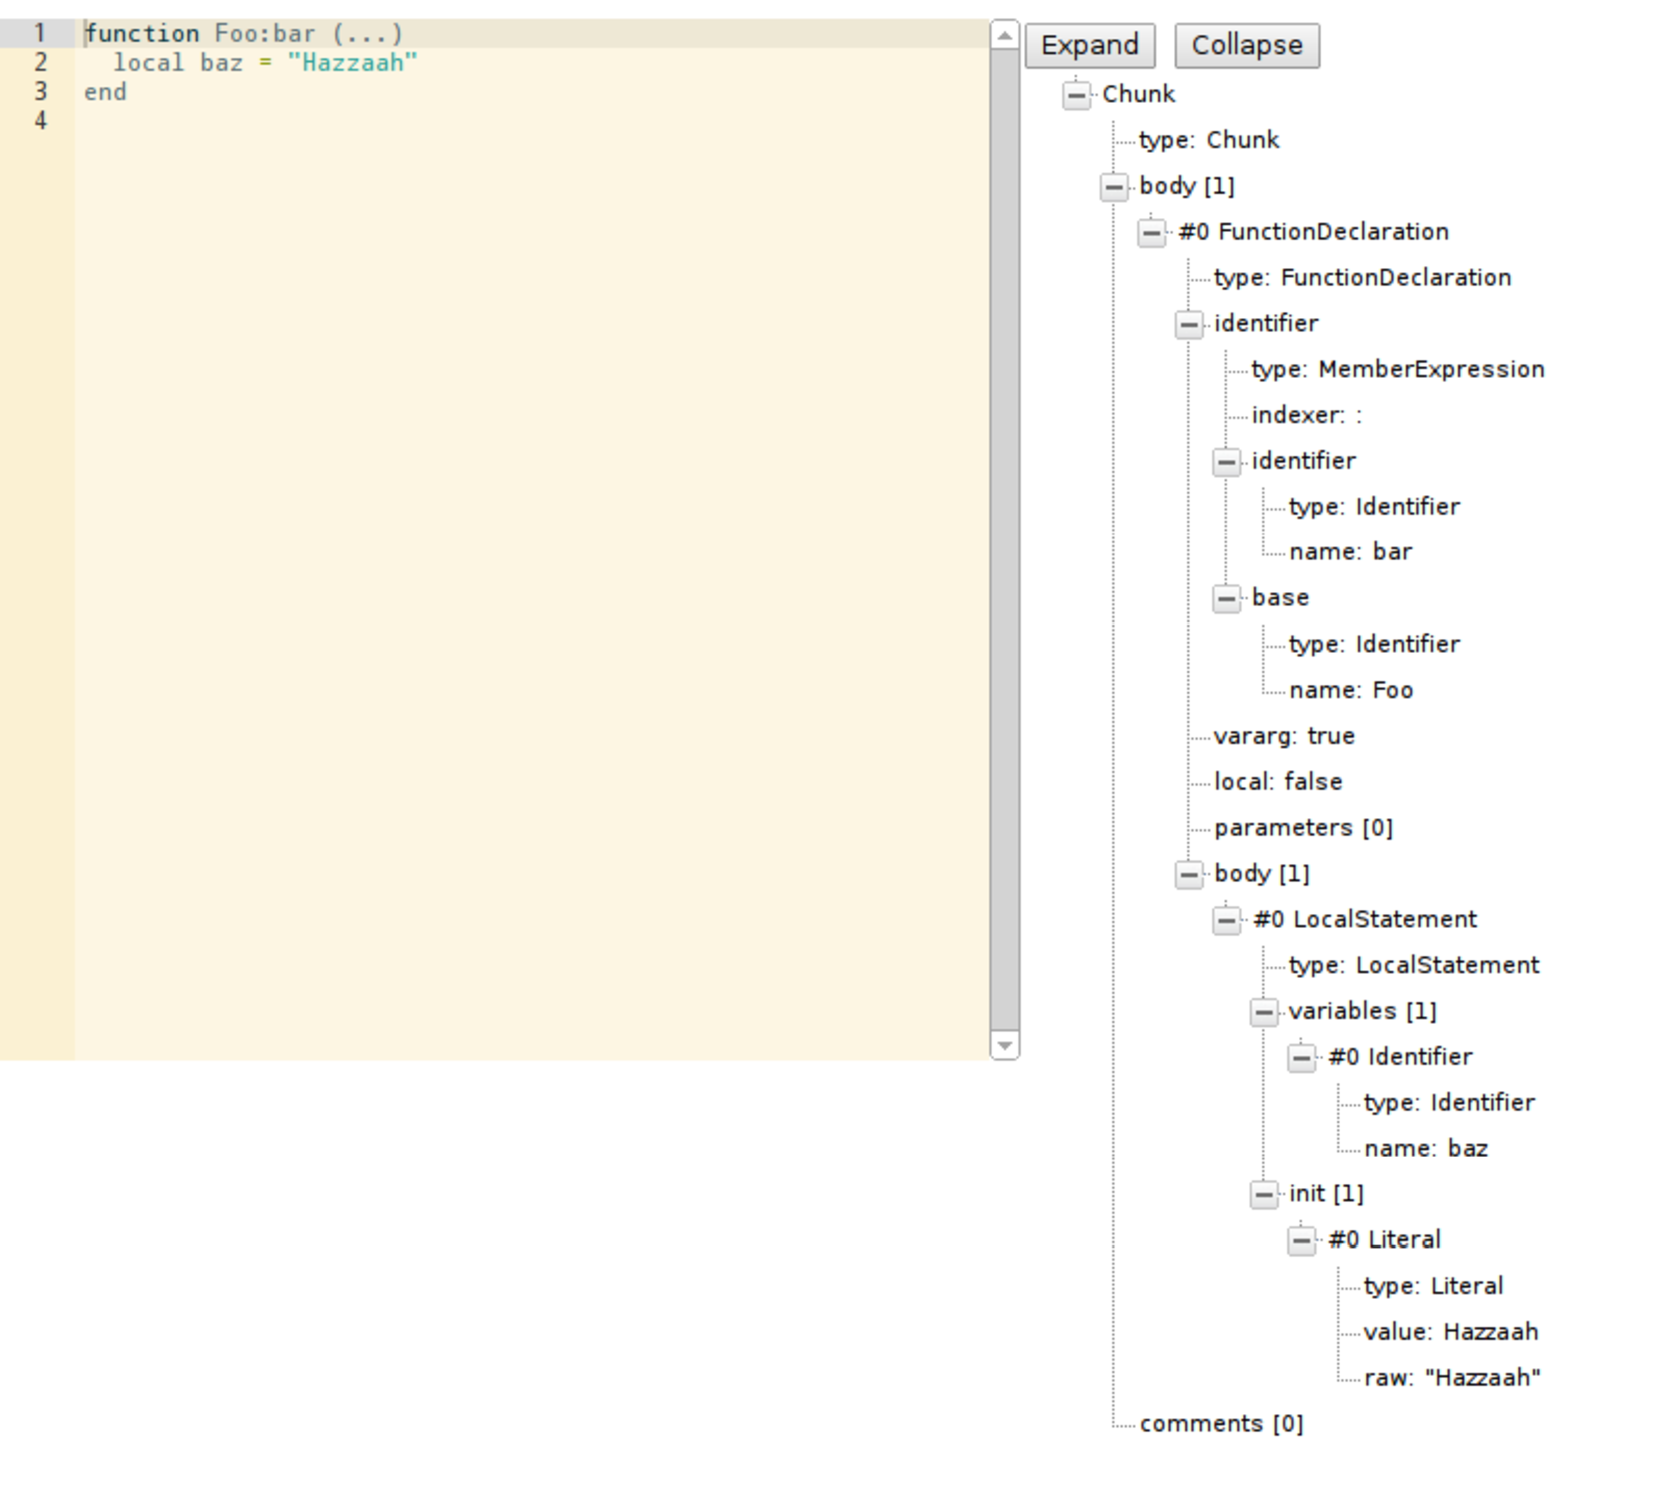
\includegraphics[width=\textwidth]{figures/pdf/tool.pdf}
  \caption{Abstrakt syntaxträd (höger) för parsningen av en Lua-funktion
  (vänster).}
  \label{fig:tool}
\end{figure}

% vim: set tw=78:ts=2:sw=2:et:fdm=marker:wrap:wm=78:ft=tex
% vim: spell spelllang=sv

\clearpage
\section{Prestandaoptimering}

Eftersom JavaScript är ett tolkat språk som evaluerar kod vid exekvering bör
tolkade språk fokusera mer tid på prestandaoptimering än kompilerade språk. Dessutom är
JavaScript ett språk som huvudsakligen körs i webbläsare med varierande
prestanda. Mindre applikationer med ett fåtal funktionsanrop behöver vanligen
inte prioritera prestandaoptimering eftersom webbläsarens JavaScript-motor är
tillräkligt effektiv för att inte påverka användarupplevelsen. Målet med detta
examensarbete handlar dock om att implementera en parser som kan användas i
nätbaserade kodredigerare, exempelvis som en \textit{``syntax highlighter''}.
Eftersom en \textit{``syntax highlighter''} behöver uppdateras vid varje
kodförändring kan antalet funktionsanrop snabbt stiga och påverka
användarupplevelsen. När användaren gör en uppdatering förväntas en omedelbar
respons och därmed måste en parser ämnad för webbläsare uppfylla detta krav.

Insamligen av data utgörs av att parsa ett exempelprogram vid specifika
revisioner av implementation. Utgående från resultatet uppdateras
implementationen och det nya resultatet granskas.

\subsection{JavaScript-motorn V8}

För att möjliggöra automation av provtaging utförs dessa test med Node.js
som använder sig av JavaScript-motorn V8. V8 är en JavaScript-motor med öppen
källkod som skapats av Google ämnad för deras webbläsare Google Chrome.

V8 består av en optimeringskompilator kallad Crankshft. Syftet med denna
kompontent är att identifiera och optimera enbart de funktioner som är
väsentliga för exekveringen av JavaScript-kod. Processen att optimera kod i en
tolk är tidskrävande och därmed bör optimeringen enbart fokusera på funktioner
som har en inverkan på exekveringstiden.

Processen för Crankshaft utgörs av fyra steg där det första innebär att
baskompilatorn kompilerar koden som normalt. Efter detta börjar en s.k.
\textit{``runtime-profiler''} övervaka körningen av programmet för att
identifiera de väsentliga funktionerna. När en funktion anses vara väsentlig
för exekveringen börjar en s.k. girig omkompilering.

En girig kompilering innebär att kompilatorn inte bryr sig om ifall
optimeringen kommer att lyckas eller inte. Istället för att analysera koden
väljer kompilatorn att testa sig fram och sedan återgå till den ursprungliga
koden om optimeringen misslyckades \citep{mk10}. Denna åtgärd kallas för
avoptimering och inträffar aktivt i körningen av JavaScript eftersom språket
är dynamiskt och en avoptimering sker varje gång en datatyp konverteras.
Ytterligare existerar det specifika strukturer som kompilatorn inte kan
optimera, exempelvis try-satser samt vissa typer av switch-satser. Även här
måste en avoptimering ske men för dessa struktur-relaterade problem kallas det
för en s.k. \textit{``bailout''}.

För att identifiera dessa avoptimeringar och \textit{``bailouts''} har V8 diverse
kommandoradsflaggor som kan användas. Dessa kan även användas för att
inspektera funktionsanrop och händelseförlopp.

\subsubsection{Kommandoradsflaggor}

Nedan följer en lista på de kommandoradsflaggor som används i detta kapitel
\citep{v8profiler}.

\begin{description}
  \item[--prof] \hfill \\
    Skapar en v8.log fil bestående av provtagning från JavaScript-stacken
    samt C++-stacken. Med hjälp av verktyget tick-processor som följer med V8
    kan användaren skapa en översikt av denna information. Översikten återger
    hur stor andel av den totala exekveringen som utgörs av varje funktion.
  \item[--trace_bailout] \hfill \\
    Anger orsaken till varför en funktion avoptimerats med en
    \textit{``bailout''}.
  \item[--trace_inlining] \hfill \\
    Registrerar varje gång en Crankshaft försöker omkompilera en funktion med
    hjälp av en teknik som kallas \textit{``function inlining''}. Denna
    optimeringsteknik innebär att kompilatorn ersätter ett funktionsanrop med
    själva funktionsinnehållet och därmed sparar kostnaden av själva andropet
    samt dess returnering. När en \textit{``function inlining''} utförs
    möjliggör det ytterligare optimeringsmöjligheter eftersom koden nu är mer
    kompakt och introducerar satser som möjligen kan kombineras med omliggande
    kod.
\end{description}

\subsection{Provtagning}

Följande moment har genomförts för att optimera prestandan av parsern fram
till att resultatet har en relativ förbättring större än 10\%. Alla test har
utförts på en dual-core 2.6 GHz dator med ett Linux-baserat operativsystem.

\subsubsection{Undvikandet av ``bailouts''}

Trots att \textit{``bailouts''} möjliggör en allmän prestandaförbättring hos
V8 är det klokt att undvika avoptimeringen eftersom den kostar en del
prestanda och kommer att återupprepas vid varje exekvering.

Genom att analysera resultatet från en parsning med kommandoradsflaggan
\textit{--trace_bailout} i bilaga 6 kan två
\textit{``bailout''}-avoptimeringar utläsas.  Funktionerna som orsakat dessa
är \textit{isUnary()} samt \textit{parsePrimaryExpression()} som bägge
innehåller en ooptimerbar switch-sats. \mbox{Node.js} v0.8.16 har inte
möjlighet att optimera funktioner som innehåller en switch-sats med
icke-litterala labels, d.v.s. variabler.

Detta är ett enkelt problem att lösa eftersom avoptimeringen inte sker för
``if-sats''-motsvarigheten och därmed kan koden optimeras enligt
\nobreak{figur~\ref{fig:bailout}}.

\lstloadlanguages{JavaScript}
\begin{figure}[ht]
  \begin{minipage}[t]{0.5\textwidth}
    \lstinputlisting[title="",language=Javascript]%
      {figures/tex/bailout-pre.js}
  \end{minipage}%
  \begin{minipage}[t]{0.5\textwidth}
    \lstinputlisting[title="",language=Javascript]%
      {figures/tex/bailout-post.js}
  \end{minipage}
  \caption{Förändring av funktionen isUnary från icke-optimerbar (vänster) till
    optimerbar (höger).}
  \label{fig:bailout}
\end{figure}

\subsubsection{Teckenkoder istället för reguljära uttryck}

Genom att analysera resultat i bilaga 7 som fås från provtagningsverktyget i
V8 framgår det att 53.5\% av en hel exekvering går åt till reguljära uttryck
som används för att identifiera blanksteg och giltiga identifierare.

Tidigare prestandamätningar \citep{charcodeat} visar ytterligare att
jämförelser på teckenkoder istället för på teckensträngar kan vara mer än dubbelt
snabbare. Orsaken för denna prestandaskillnad är att JavaScript-motorn
utnyttjar binära operationer när den jämför teckenkoder. På grund av denna
prestandaskillnad ersätts reguljära uttryck med switch- och if-satser som
jämför teckenkoder.

\subsubsection{Optimering av sträng-funktioner}

Efter att de tidigare optimeringarna genomförts betonas nu 2 huvudsakliga
funktioner i provtagningsanalysen i bilaga 8. Dessa funktioner, dvs.
\textit{StringAddStub} som är en maskinkodsmetod för att sammanfoga strängar
och \textit{CompareICStub} som är en maskinkodsmetod för att jämföra strängar,
upptar 20\% av parsningsprocessens exekveringstid.

\textit{StringAddStub} orsakas av att lexern sammanfogar token-värden för
kommentarer, tal och identifierare genom att iterera över varje tecken så
länge som en avgränsare inte påträffas. Denna procedur går att förenkla genom
att istället memorera var värdet börjar och sedan iterera fram till
avgränsaren. När avgränsaren hittats kan värdet identifieras från dess
startposition till dess avgränsare enligt exemplet i figur~\ref{fig:stringAddStub}.

\lstloadlanguages{JavaScript}
\begin{figure}[ht]
  \begin{minipage}[t]{0.5\textwidth}
    \lstinputlisting[title="",language=Javascript]%
      {figures/tex/stringaddstub-pre.js}
  \end{minipage}%
  \begin{minipage}[t]{0.5\textwidth}
    \lstinputlisting[title="",language=Javascript]%
      {figures/tex/stringaddstub-post.js}
  \end{minipage}
  \caption{Optimering av vänstra funktionens strängsammanfogning till högra
    funktionens identifiering.}
  \label{fig:stringAddStub}
\end{figure}

Orsaken till den långsamma \textit{CompareICStub}-operationen visar sig vara
en \textit{``function inlining''} i uttrycksparsern. Funktionen ansvarar för
att ange prioriteten av en given operator utgående från en switch-sats
med strängjämförelser. Eftersom funktionen körs för varje uttryck som hittas
valde jag att uppoffra läsligheten med att istället jämföra teckenkoder en
efter en enligt figur~\ref{fig:switchtree}. Efter att optimeringen
gjorts valideras ännu att funktionen är tillräkligt liten för
\textit{``function inlining''}, vilket den visar sig vara.

\begin{figure}[ht]
  \begin{minipage}[t]{0.5\textwidth}
    \lstinputlisting[title="",language=Javascript]%
      {figures/tex/prefixtree-pre.js}
  \end{minipage}%
  \begin{minipage}[t]{0.5\textwidth}
    \lstinputlisting[title="",language=Javascript]%
      {figures/tex/prefixtree-post.js}
  \end{minipage}
  \caption{Optimering från jämförelse av tecken (vänster) till jämförelse av teckenkoder (höger).}
  \label{fig:switchtree}
\end{figure}

\subsection{Resultat}

Efter optimeringarna i detta kapitel har de huvudsakliga flaskhalsarna
avlägsnats från parsern. En överblick av exekveringstiden för de nuvarande
funktionerna visas i figur~\ref{fig:funcdist}. Funktionerna
\textit{readToken()} och \textit{scanIdentifierOrKeyword()} som kräver mest
exekveringstid är redan optimerade och kan inte förbättras.

\begin{figure}[ht]
  \includegraphics[width=13cm]{figures/output/functions.pdf}
  \caption{Slutgiltig översikt av exekveringstiden för parser-implementations
    funktioner.}
  \label{fig:funcdist}
\end{figure}

En översikt av förbättringsskillnaderna från kapitlets prestandaoptimeringar
visas i figur~\ref{fig:perf-overview}.

\begin{figure}[ht]
  \includegraphics[width=13cm]{figures/output/commits.pdf}
  \caption{Översikt av moment i.o.m. parser-implementationens
    prestandaoptimering.}
  \label{fig:perf-overview}
\end{figure}

% vim: set tw=78:ts=2:sw=2:et:fdm=marker:wrap:wm=78:ft=tex
% vim: spell spelllang=sv

\clearpage
% \section{Kvalitetsanalys}

\subsection{Mätning}

\subsubsection{Test}

\subsubsection{Kodtäckning}

\subsubsection{Kod komplexitet}

\subsubsection{Benchmark}

\subsection{Automation}

\subsubsection{Kontinuerling integration}

\subsubsection{Git hook}

\subsection{Jämförelse med liknande parsers}

\begin{figure}[ht]
  \includegraphics[width=13cm]{figures/output/parsers.pdf}
  \caption{Jämförelse av parser-implementationen och andra liknande lösningar}
\end{figure}


% \clearpage
\section{Diskussion och slutsatser}

Slutresultatet av detta examensarbete är en prestandaoptimerad rekursivt
nedstigande parser av Lua-språket. Implementationen av parsern är en pågående
process som påbörjats 6 månader innan detta examensarbete fullgjorts.

Tidsmängden krävd för implementationen är omöjlig att mäta, men resultatet
utgörs av mer än 1600 källkodsrader samt mer än 600 logiska programkodsrader.
Ytterligare existerar det mer än 500 test som används för att upprätthålla
parserns kvalitet. I efterhand kan jag konstatera att implementationen varit
en okomplicerad men tidskrävande process. Eftersom tidsmängden för att
generera en Lua-parser med hjälp av Jison enbart tog enstaka timmar är
skillnaden mellan implementationsalternativen enorm. Slutprodukten visar sig
dock vara en stabil och prestandaeffektiv implementation som kan användas i
praktiken. Likt skaparna av GCC och Lua anser jag inte tidsmängden vara för
mycket när det handlar om ett språk med en stabil och enkel syntax. Fördelen
som fås visas tydligt i dess prestanda, dess felmeddelanden och enkelheten av
källkoden.

För språk med en mer komplicerad syntax såsom C++ eller PHP anser jag dock
inte det vara möjligt att upprätthålla en handskriven parser. Dessutom sker
det kontinuerligt uppdateringar i syntaxen av ett språk, vilket vi kan se i
senaste versionen av PHP samt i den uppkommande versionen av JavaScript.
Processen att uppdatera syntaxgrammatiken för en genererad parser innebär
enbart justeringar i en grammatikspecifikation. I en handskriven parser kan
det innebära stora strukturella förändringar.

Slutsatsen jag har är att projekt som körs i en prestandakritisk miljö med ett
tolkat språk bör överväga att implementera en handskriven parser. Om
tidsmängden är begränsad eller projektet inte är prestandakritiskt kan dock en
maskingenererad parser användas.

Det finns fortfarande en serie förbättringar som kan göras till denna
parser för att vara mer användbar som ett analyseringsverktyg. I nästa version
har jag planer att introducera inkrementell parsning så att syntaxmarkerare
inte behöver parsa en hel fil för att göra uppdateringar. Ytterligare planerar
jag anknyta källdkodspositionen till varje nod i syntaxträdet för att ett
verktyg lättare skall kunna manipulera programkod.

Slutprodukten av arbetet finns i \url{http://oxyc.github.io/luaparse/} och är
licenseriad under MIT-licensen. Implementationen kan användas med Node.js
eller en webbläsare med en JavaScript-motor som implementerats enligt ECMA-262
version 3.

% vim: set tw=78:ts=2:sw=2:et:fdm=marker:wrap:wm=78:ft=tex
% vim: spell spelllang=sv



% Inledning
% - Målsättning och syfte
% - Utförande
% - Begränsningar
% - Definitioner
%
% Programmeringsspråk
% - Flöde
% - Kontextfri grammatik
%   - Backaus-Naur Form
% - Lua
%   - ..
%
% Parser teknologi
% - Lexikalisering
%   - Scanner
%   - Tokenizer
% - Syntastisk analys
%   - AST
% - Patterns
%   - Recursive descent
%   - Bottom-up
% - Parser Generators
%
% Parser implementation
% - Krav
% - Verktyg
% - Analys av Lua
% - Parser design
% - Algoritm optimering
%
% Diskussion


% Include the reference list
\bibliography{references}

% Include your appendices
\newpage
\thispagestyle{empty}
\appendix
\addcontentsline{toc}{section}{Bilaga - Källkod}
\section*{Bilaga - Lua grammatik}

\begin{grammar}
  \singlespace\small%
  \fontfamily{lmr}\selectfont

  <chunk> ::= <block>

  <block> ::= \{<stat>\} [<retstat>]

  <stat> ::=  ";"
     \alt <varlist> "=" <explist>
     \alt <functioncall>
     \alt <label>
     \alt "break"
     \alt "goto" Name
     \alt "do" <block> "end"
     \alt "while" <exp> "do" <block> "end"
     \alt "repeat" <block> "until" <exp>
     \alt "if" <exp> "then" <block> \{"elseif" <exp> "then" <block>\} ["else" <block>] "end"
     \alt "for" Name "=" <exp> "," <exp> ["," <exp>] "do" <block> "end"
     \alt "for" <namelist> "in" <explist> "do" <block> "end"
     \alt "function" funcname <funcbody>
     \alt "local" <function> Name <funcbody>
     \alt "local" <namelist> ["=" <explist>]

  <retstat> ::= "return" [<explist>] [";"]

  <label> ::= "::" Name "::"

  <funcname> ::= Name \{"." Name\} [":" Name]

  <varlist> ::= <var> \{"," <var>\}

  <var> ::= Name | <prefixexp> "[" <exp> "]" | <prefixexp> "." Name

  <namelist> ::= Name \{"," Name\}

  <explist> ::= <exp> \{"," <exp>\}

  <exp> ::=  "nil" | "false" | "true" | Number | String | "..." | <functiondef> |
     <prefixexp> | <tableconstructor> | <exp> <binop> <exp> | <unop> <exp>

  <prefixexp> ::= <var> | <functioncall> | "(" <exp> ")"

  <functioncall> ::=  <prefixexp> <args> | <prefixexp> ":" Name <args>

  <args> ::=  "(" [<explist>] ")" | <tableconstructor> | String

  <functiondef> ::= "function" <funcbody>

  <funcbody> ::= "(" [<parlist>] ")" <block> "end"

  <parlist> ::= <namelist> ["," "..."] | "..."

  <tableconstructor> ::= "\{" [<fieldlist>] "\}"

  <fieldlist> ::= <field> \{<fieldsep> <field>\} [<fieldsep>]

  <field> ::= "[" <exp> "]" "=" <exp> | Name "=" <exp> | <exp>

  <fieldsep> ::= "," | ";"

  <binop> ::= "+" | "-" | "*" | "/" | "\textasciicircum" | "\%" | ".." |
     "<" | "<=" | ">" | ">=" | "==" | "~=" |
     "and" | "or"

  <unop> ::= "-" | "not" | "\#"
\end{grammar}

\section*{Bilaga - Källkod}


\end{document}

% vim: set tw=78:ts=2:sw=2:et:fdm=marker:wrap:wm=78:ft=tex
